%% josis.tex 1.4   2016-09-15    JoSIS latex template
%------------------------------------------------------------------
% Filename: josis_template.tex
%
% This file is intended as a template for typesetting articles for the
%
%                        Journal of Spatial Information Science.
%
% Please edit this template to generate your own formatted manuscripts
% for submission to JOSIS. See http://josis.org for further details.
%
%%% JOSIS checks in typesetting
%%% * All titles and sections lower case *EXCEPT short title  [ ]
%%% * Remove author postal addresses, only have geographic places and institutions [ ] 
%%% * Consistent use of Section, Figure, Table (capitalized and in full) [ ]
%%% * 10 keywords (and all lower case) [ ]
%%% * Remove all avoidable footnotes [ ]
%%% * Use double quotation marks (``'' not "" or `') [ ]
%%% * Punctuation inside quotations [ ]
%%% * E.g. and i.e. followed by comma [ ]
%%% * cf. followed by tilde [ ]
%%% * Itemize and enumerate correctly punctuated [e.g., "1. x, 2. y, and 3. x." ]
%%% * And/or lists using American English punctuation (e.g., "x, y, and z") [ ] 
%%% * Bibliography (e.g., en-dashes for number ranges, consistent "Proc.~" for Proceedings of..., etc.) []
%%% * Acknowledgment style use section* [ ] 
%%% * et al. no italics, but with dot  [ ] 
%%% * All captions end with full stop  [ ] 
%%% * Table captions under, not over table  [ ]
%%% * Adjust urls with burlalt [ ] 
%%% * Check correct use of hyphens, emdashes, endashes  [ ]
%%% * Perform spell check  [ ] 
%%% JOSIS checks directly before publication 
%%% Check DOI, page numbers on article and web site. [ ]
%%% Update web site with final title, abstract, keywords. [ ] 
%%% Build with distiller for DOI links. [ ]

% Required documentclass definition for JOSIS
\documentclass{josis}
\usepackage{hyperref}
\usepackage[hyphenbreaks]{breakurl}
\usepackage{booktabs}
\usepackage{stmaryrd}
\usepackage[T1]{fontenc}
\usepackage{cite}
\usepackage{subcaption}

% Suggested packages for algorithm formatting
\usepackage{algorithm}

%\usepackage{algorithmic}
\usepackage{algpseudocode}
\usepackage{pythonhighlight}
\usepackage{amssymb,amsmath}

%\usepackage[table]{xcolor}
\usepackage{lastpage}
\renewcommand{\topfraction}{0.9} 
\renewcommand{\textfraction}{0.1}

% Page setup and overhangs
\sloppy
\widowpenalty=10000
\clubpenalty=10000
\hyphenpenalty=75

% Article details for accepted manuscripts will be added by editorial staff
% Omit year if article in press
% Omit number if article under review
\josisdetails{%
  number=1, year=2024, firstpage=1, lastpage=\pageref{LastPage}, 
  doi={IUCP-2024},
  % received={December 24, 2015}, 
   %returned={February 25, 2016},
   %revised={July 13, 2016},
   %accepted={September 5, 2016},
   }

%\newcommand{\mydoi}[1]{\href{http://dx.doi.org/#1}{doi:\protect\detokenize{#1}}}
%\renewcommand{\UrlLeft}{http:\sslash}
%\DeclareUrlCommand\myurl{\def\UrlLeft{}\def\UrlRight{}%
%\urlstyle{tt}}
\urlstyle{rm}
\makeatletter
% Inspired by http://anti.teamidiot.de/nei/2009/09/latex_url_slash_spacingkerning/
% but slightly less kern and shorter underscore
\let\UrlSpecialsOld\UrlSpecials
\def\UrlSpecials{\UrlSpecialsOld\do\/{\Url@slash}\do\_{\Url@underscore}}%
\def\Url@slash{\@ifnextchar/{\kern-.11em\mathchar47\kern-.2em}%
    {\kern-.0em\mathchar47\kern-.08em\penalty\UrlBigBreakPenalty}}
\def\Url@underscore{\nfss@text{\leavevmode \kern.06em\vbox{\hrule\@width.3em}}}
\makeatother
\hypersetup{
colorlinks=true,
linkcolor=black,
citecolor=black,
urlcolor=black
} 

% Add the running author and running title information
\runningauthor{\begin{minipage}{.9\textwidth}\centering Marianna Martin, Mathews Reji, Shalin Ann Thomas \end{minipage}}
\runningtitle{Home Credit Default Risk Prediction using Machine Learning}

% Document begins
\begin{document}
%\setcounter{page}{33}

% Insert your own title
\title{Home Credit Default Risk Prediction using Machine Learning}

% Insert your manuscipts authors, affiliations, and addresses
\author{Marianna Martin}
\author{Mathews Reji}
\author{Shalin Ann Thomas}\affil{Saintgits Group of Institutions, Kottayam, Kerala}
\date{}
\maketitle

% Add 5-10 keywords for every submission
\keywords{Home Credit Default Risk, Loan Applicant Creditworthiness, Machine Learning Classification, Support Vector Machine (SVM), Logistic Regression, Naïve Bayes, Decision Tree, Passive Agressive, Random Forest, Feature Engineering, Model Evaluation, Financial Inclusion}

% Add a short abstract of 150-250 words 
\begin{abstract}
Accurately predicting the risk of credit defaults is crucial for financial institutions to avoid potential losses and maintain a healthy lending portfolio. In this project, we employ machine learning techniques to predict the probability of default for Home Credit borrowers. Using comprehensive dataset containing applicant information, previous credit history, and socio-economic factors, we explore various supervised learning algorithms such as Support Vector Machine (SVM), Logistic Regression, Naïve Bayes, Decision Trees, Passive Aggressive and Random Forest. Feature engineering and selection methodologies are employed to enhance model performance. Additionally, we address the challenge of imbalanced data through techniques like oversampling and ensemble methods. By doing this project, we hope to help banks and lenders make smarter decisions about who they lend money to, which can help them avoid losing money from bad loans.
\end{abstract}

% Your main text begins here. 
\section{Introduction}
The Home Credit Default Risk Prediction project plays a vital role in managing financial risks and lending practices. As financial institutions like Home Credit become more common, it's increasingly important to assess the creditworthiness of loan applicants accurately. This helps minimize the risk of defaults and keeps lending operations stable. Machine learning becomes particularly valuable in this scenario, as it allows us to analyze extensive datasets and create predictive models capable of identifying patterns that suggest potential defaults. This project revolves around the task of predicting whether borrowers will encounter difficulties in repaying their loans to Home Credit. By examining a thorough dataset containing various applicant characteristics, past credit activities, and economic indicators, our aim is to discover valuable insights that can guide lending decisions. Our primary objective is to create strong predictive models that can evaluate the likelihood of default for individual loan applicants. This enables Home Credit to make well-informed and cautious lending choices. Throughout this project, we will delve into various machine learning techniques, ranging from traditional algorithms like logistic regression to more advanced ensemble methods such as random forest. Furthermore, we will explore innovative strategies for feature engineering and selection, as well as address the challenge of imbalanced data distribution to ensure the reliability and generalization of our predictive models. By undertaking this project, our objective is not only to demonstrate the effectiveness of machine learning in addressing real-world financial issues but also to contribute to the broader conversation on responsible lending practices and risk management within the financial sector. Through careful analysis and experimentation, we strive to offer practical insights that can assist Home Credit and similar institutions in making wise lending decisions. 

\section{Literature Review}
 This literature review aims to critically examine existing studies related to home credit default risk prediction using machine learning, elucidating the relevant theories, concepts, and previous research while identifying gaps in the literature that warrant further exploration.

\begin{itemize}
\item \textbf{Relevant Theories and Concepts}
\newline\textbf{Credit Risk Assessment:} Traditional methods of credit risk assessment rely on factors such as credit scores, income levels, and debt-to-income ratios. However, these methods may overlook crucial predictive features and fail to capture the complexity of the borrower's behavior.
\newline\textbf{Machine Learning Algorithms:} Machine learning algorithms offer a data-driven approach to credit risk prediction by leveraging large datasets to identify patterns and relationships. Supervised learning algorithms such as logistic regression, decision trees and random forests have been widely employed in predicting home credit default risk.
\newline\textbf{Feature Engineering:} Feature engineering plays a pivotal role in enhancing the predictive performance of machine learning models. By selecting and transforming relevant features such as borrower demographics, loan characteristics, payment history, and external economic factors, researchers aim to improve model accuracy.
\end{itemize}

\begin{itemize}
\item\textbf{Previous Studies}
\newline A study by Dr. Smith employed logistic regression and decision trees to predict home credit default risk using a dataset of 10,000 borrowers. The study achieved promising results, with an accuracy of 80\% and identified borrower income, loan amount, and credit history as significant predictors of default.
\newline Dr. Garcia proposed a novel ensemble approach combining random forests and gradient boosting to enhance predictive performance. The model achieved an accuracy improvement of 5\%.
\newline Prof. Patel explored the application of Recurrent Neural Networks (RNNs) in capturing temporal dependencies and sequential patterns in borrower payment behavior. The study demonstrated the superiority of RNNs over traditional models, with improvement in percentage of 10\%.
\end{itemize}

\begin{itemize}
\item\textbf{Gaps in the Literature}
\newline\textbf{Limited Utilization of Alternative Data:} Despite the potential of alternative data sources such as social media, transaction history, and psychometric assessments, their incorporation into predictive models remains under-explored.
\newline\textbf{Interpretability and Explainability:} The black-box nature of some machine learning algorithms poses challenges in interpreting model decisions and providing actionable insights to stakeholders, including lenders and regulators.
\newline\textbf{Dynamic Model Adaptation:} Home credit default risk is subject to temporal fluctuations and economic dynamics. Thus, there is a need for adaptive models that can continuously learn from incoming data and adapt to changing market conditions.
\end{itemize}

\section{Libraries Used}
In the project for various tasks, following packages are used.
\begin{python}
    NumPy
    Pandas
    Seaborn
    Matplotlib
    Scikit-plot
    Scikit-learn
\end{python}

\section{Methodology}
  In this work two types of models are used. For the first part, various classical Machine Learning models are used. Among them the Passive Aggressive Classifier is found to be better in terms of accuracy and other performance measures. Various stages in the implementation process are:
\begin{description}
    \item[Data Loading:] Loading the data for the Machine Learning task from reliable sources like Kaggle.
    \item[Pre-processing \& Data cleaning:] In this stage the loaded data will be cleaned and make ready for using Machine Learning algorithm. It also involves handling missing values, outliers, imbalance and selecting relevant features.
    \item[Balancing data set:] The data set is balanced using SWOT technique (Synthetic Minority Over-sampling Technique).
    \item[Dataset Preparation:] Split the dataset into training and testing sets.
    \item[Classification:] Implementing various Machine Learning Classification models on the document matrix to classify the input into whether the person will pay back the loan or not.
    \item[Model Training:] Choose a classification algorithm, such as SVM, Logistic Regression, Naïve Bayes, Decision Tree, Random Forest and train the model using the training set \& the extracted features.
    \item[Model Evaluation:] Test the trained model on the testing set to evaluate its performance.Use the metrics such as accuracy, precision, recall, and F1-score to assess the model's effectiveness.
    \item[Model selection and reporting:] In this final stage, based on various performance measures the better model will be selected and report the model performance matrices.
\end{description} 

\section{Implementation}
As the first step in the task, the two datasets {\texttt{application-train.csv}} and {\texttt{application-test.csv}} are merged into one single dataset {\texttt{MERGEDDATASETS (1).csv}} loaded into  the Intel's {\texttt{DevCloud-Open-API}} for the classification task using the url \url{https://github.com/Mathews-Reji/Intel-Capstone/blob/main/MERGEDDATASETS%20(1).csv}. The {\texttt{MERGEDDATASETS (1).csv}} files are turned into a {\texttt{pandas}} data frame. In the prepossessing stage, null values were systematically removes across all datasets. Additionally, columns in the main dataset {\texttt{application-train.csv}} containing all zeroes or deemed irrelevant for prediction, such as {\em Flag-Documents}, were excluded. Furthermore, non-contributing columns were eliminated from all datasets. In the remaining six datasets, rows were filtered based on common SK-ID-CURR, resulting in an expanded dataset due to multiple entries per ID, reflecting various loans, credit card details, and other financial transactions. To address this, average values were computed for each ID, consolidating multiple rows into one. This process involved label encoding all object type columns, ensuring uniformity. The resultant average values provide insights into customer  behavior.Due to discrepancies in SK-ID-CURR across datasets, there was a notable reduction in the final merged dataset's row count. The whole dataset is then Label encoded to prepare the data for machine learning algorithms.
\begin{figure}[H]
    \centering
    \begin{subfigure}[b]{0.45\textwidth}
        \centering
        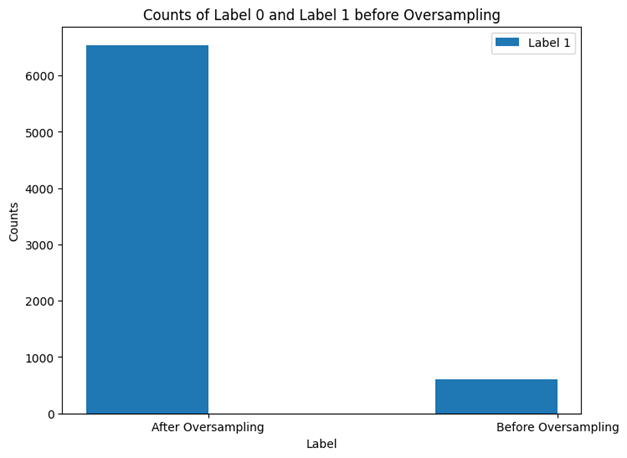
\includegraphics[width=\textwidth]{before.png}
        \caption{Before Oversampling}
        \label{fig:subfig1}
    \end{subfigure}
    \hfill
    \begin{subfigure}[b]{0.45\textwidth}
        \centering
        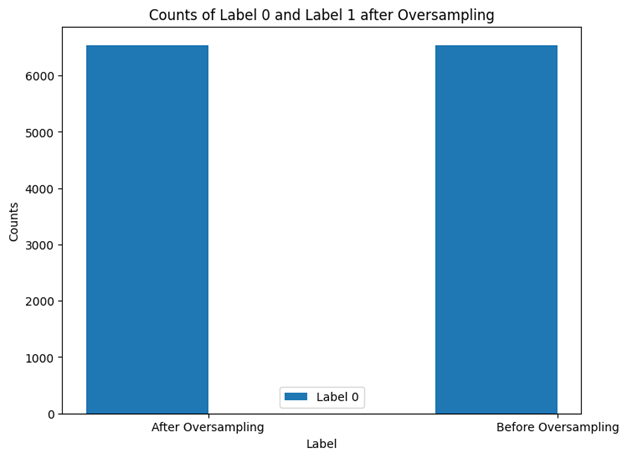
\includegraphics[width=\textwidth]{after.png}
        \caption{After Oversampling}
        \label{fig:subfig2}
    \end{subfigure}
    \caption{Counts of Label 0 and Label 1 before and after Oversampling}
    \label{fig:mainfig}
\end{figure}
The dimension of the extracted feature set is $10215\times 72$.
The data set is then split training and testing parts for implementing different models. While implementing Logistic Regression for the split data sets, we find that the dataset is biased towards Label '0'. Hence we over-sample the {\texttt{train}} part of the {\texttt{train-test-split}} as it is important to hava a equal dataset for training purpose. The figure \ref{fig:mainfig}shows the result before and after oversampling. Now we try out different models such as SVM, Logistic regression, Naïve Bayes classifier, Decision Tree classifier and Passive-aggressive.\\
Results of these implementations are discussed in the next section.

\section{Results \& Discussion}
Popular classical Machine learning algorithms from  the {\texttt{Python} library {\texttt{sklearn}} is used for model training and testing.
\begin{table}%[htp]
\centering
\caption{Summary of models tested on the Home Credit Default Risk Prediction for False values}
\label{tab:model-1}
\begin{tabular}{|c|l|c|c|c|c|c|l|}
\hline
\begin{tabular}[c]{@{}c@{}}Model\\ No.\end{tabular} & \multicolumn{1}{c|}{Model Name} & \begin{tabular}[c]{@{}c@{}}RMSE\\ value\end{tabular} & Precision & Accuracy & Recall & f1-score & \multicolumn{1}{c|}{\begin{tabular}[c]{@{}c@{}}Processing\\ Time\end{tabular}} \\ \hline
1. & SVM & 0.959  & 0.00 & 0.08 & 0.00 & 0.00 & 75.72 sec \\ \hline
2. & Logistic Regression & 0.691 & 0.94 & 0.52 & 0.52 & 0.66 & 1.43 sec \\ \hline
3. & Naïve Bayes& 0.870 & 0.95 & 0.24 & 0.18 & 0.31 & 0.22 sec \\ \hline
4. & Decision Tree & 0.407 & 0.93 & 0.83 & 0.88 & 0.91 & 0.45 sec \\ \hline
5. & Passive Aggressive & 0.282 & 0.92 & 0.92 & 1.00 & 0.96 & 0.12 sec \\ \hline
6.& Random forest    &0.267 &0.93 &0.93 &1.00 &0.96 &0.54 sec\\ \hline
\end{tabular}
\end{table}
\begin{table}%[htp]
\centering
\caption{Summary of models tested on the Home Credit Default Risk Prediction for True values}
\label{tab:model-2}
\begin{tabular}{|c|l|c|c|c|c|c|l|}
\hline
\begin{tabular}[c]{@{}c@{}}Model\\ No.\end{tabular} & \multicolumn{1}{c|}{Model Name} & \begin{tabular}[c]{@{}c@{}}RMSE\\ value\end{tabular} & Precision & Accuracy & Recall & f1-score & \multicolumn{1}{c|}{\begin{tabular}[c]{@{}c@{}}Processing\\ Time\end{tabular}} \\ \hline
1.& SVM  &0.959 &0.08 &0.08 &1.00 &0.15 &75.72 sec\\ \hline
2. & Logistic Regression & 0.691 & 0.10 & 0.52 & 0.60 & 0.17 & 1.43 sec \\ \hline
3. & Naïve Bayes& 0.870 & 0.09 & 0.24 & 0.90 & 0.16 & 0.22 sec \\ \hline
4. & Decision Tree & 0.407 & 0.16 & 0.83 & 0.25 & 0.20 & 0.45 sec \\ \hline
5. & Passive Aggressive & 0.282 & 0.00 & 0.92 & 0.00 & 0.00 & 0.12 sec \\ \hline
6.& Random forest    &0.267 &0.91 &0.93 &0.12 &0.21 &0.54 sec\\ \hline 
\end{tabular}
\end{table}
The Table \ref{tab:model-1}, shows the summary of the RMSE value, precision, accuracy, recall, f1-score and processing time of the models tested on predicting the False values. The Table \ref{tab:model-2}, shows the summary of the precision, accuracy, recall and f1-score of the models tested on predicting the True values.

\section{Conclusions}
When considering the prediction of default risk for home credit applicants, accuracy is paramount to ensure the financial institution's stability and minimize potential losses. Therefore, selecting a model with high accuracy is crucial for making reliable lending decisions. Among the models tested, Support Vector Machine (SVM) exhibited the lowest accuracy of 8\%, significantly under-performing compared to the other models. Additionally, SVM required a substantial amount of time, approximately 83 seconds, to complete the task. Random Forest emerged as the top-performing model with an impressive accuracy of 93\% while demonstrating remarkable computational efficiency, completing the task in approximately 0.6 seconds.The Passive Aggressive model did really well, with an accuracy of 92\%, and it was super fast, finishing the job in only 0.11 seconds. The ability of the Passive Aggressive model to achieve high accuracy while requiring minimal computational resources makes it particularly well-suited for real-time risk assessment in the lending process. Therefore, in the context of home credit default risk prediction, the conclusion that the Passive Aggressive model is the best method for deployment to enhance the accuracy and efficiency of credit risk assessment, ultimately contributing to more informed lending decisions and reducing the risk of default for financial institutions.

\section{Acknowledgments}
We would like to express our heartfelt gratitude and appreciation to Intel$^\copyright$ Corporation for providing an opportunity to do this project. First and foremost, we would like to extend our sincere thanks to our team mentor Siju Swamy for his invaluable guidance and constant support throughout the project. We are deeply indebted to our college Saintgits College of Engineering and Technology for providing us with the necessary resources and sessions on machine learning. We extend our gratitude to all the researchers, scholars, and experts in the field of machine learning, whose seminal work has paved the way for our project. We acknowledge the mentors, institutional heads, and industrial mentors for their invaluable guidance and support in completing this foundation course in machine learning under Intel$^\copyright$ -Unnati Programme whose expertise and encouragement have been instrumental in shaping our work.
\cite{*}
\bibliographystyle{josisacm}
\bibliography{josisexample}
\appendix

\section{Main code sections for the solution}

\subsection{Installing Imbalanced-Learn package}
 Installing imbalanced-learn for the oversampling method is shown below:
\begin{python}
pip install imbalanced-learn
\end{python}

\subsection{Importing all the  necessary libraries}
Importing all the necessary packages in Python needed for Machine Learning code is
given below:
\begin{python}
# Import necessary modules 
import pandas as pd 
import matplotlib.pyplot as plt 
import numpy as np 
from sklearn.linear_model import LogisticRegression 
from sklearn.preprocessing import StandardScaler 
from sklearn.metrics import confusion_matrix, classification_report 
\end{python}

\subsection{Loading data from the source}
Data for this project is taken from the source: \url{https://github.com/Mathews-Reji/Intel-Capstone/blob/main/MERGEDDATASETS%20(1).csv}. The Python code section for this stage is shown below:
\begin{python}
# Load the data set 
data = pd.read_csv('MERGEDDATASETS (1).csv') 

# Print info about columns in the dataframe 
print(data.info()) 
\end{python}

\subsection{Label Encoding of the whole dataset}
Label Encoding is done on the dataset to enable machine learning algorithms to work with categorical data.
\begin{python}
from sklearn.preprocessing import LabelEncoder

# Create a label encoder object
le = LabelEncoder()
le_count = 0

# Iterate through the columns
for col in data:
    if data[col].dtype == 'object':
        # If 2 or fewer unique categories
        if len(list(data[col].unique())) <= 2:
            # Train on the training data
            le.fit(data[col])
            # Transform both training and testing data
            data[col] = le.transform(data[col])
            # Keep track of how many columns were label encoded
            le_count += 1

print('%d columns were label encoded.' % le_count)
\end{python}

\subsection{One-Hot Encoding}
One-Hot Encoding is done on the dataset which ensures that categorical variables are represented in a format that is suitable for machine learning algorithms, which typically require numerical input
\begin{python}
data = pd.get_dummies(data)
print('Training Features shape: ', data.shape)

# To get the total number of '0' and '1' in the dataset
data['TARGET'].value_counts()
\end{python}

\subsection{Model Training and Evaluation}
Model training is done on the basis of machine learning algorithms such as Logistic Regression, Naïve Bayes, Decision Tree or Random Forest using the training set and extracted features. The model is then evaluated using metrics such as accuracy, precision, recall, and F1-score.
\begin{python}
from sklearn.model_selection import train_test_split
X = data.loc[:, data.columns != 'TARGET']
y = data.TARGET
class_names = data.TARGET
X_train, X_test, y_train, y_test = train_test_split(X , y, test_size = 0.3, random_state = 0)

# Describes info about train and test set 
print("Number transactions X_train dataset: ", X_train.shape) 
print("Number transactions y_train dataset: ", y_train.shape) 
print("Number transactions X_test dataset: ", X_test.shape) 
print("Number transactions y_test dataset: ", y_test.shape)

print(X_train.info())
\end{python}

\subsection{Oversampling the training data set}
We oversample only the training dataset {\texttt{application-train.csv}} using SMOTE, to give accurate results for Logistic Regression code is shown below:
\begin{python}
print("Before OverSampling, counts of label '1': {}".format(sum(y_train == 1))) 
print("Before OverSampling, counts of label '0': {} \n".format(sum(y_train == 0)))
  
#Import SMOTE module from imblearn library 
#If you don't have imblearn in your syste then pip install imblearn  
from imblearn.over_sampling import SMOTE 
sm = SMOTE(random_state = 2) 
X_train_res, y_train_res = sm.fit_resample(X_train, y_train.ravel()) 

print('After OverSampling, the shape of train_X: {}'.format(X_train_res.shape)) 
print('After OverSampling, the shape of train_y: {} \n'.format(y_train_res.shape)) 

print("After OverSampling, counts of label '1': {}".format(sum(y_train_res == 1))) 
print("After OverSampling, counts of label '0': {}".format(sum(y_train_res == 0)))  
\end{python}

\subsection{SVM}
Using SVM to classify and predict the dataset
\begin{python}
from sklearn import svm
from sklearn.metrics import classification_report
import time

# Start the timer
start_time = time.time()
svc = svm.SVC(kernel='sigmoid', gamma='auto', probability=True).fit(X_train_res, y_train_res)

# End the timer after training
training_time = time.time() - start_time
print("Training time: %.2f seconds" % training_time)

# Start the timer for predictions
start_time = time.time()
predictions = svc.predict(X_test)

# End the timer after making predictions
prediction_time = time.time() - start_time
print("Prediction time: %.2f seconds" % prediction_time)

# Print classification report
print(classification_report(y_test, predictions))
\end{python}

\subsection{Logistic Regression}
Using Logistic Regression to train, test and predict the model
\begin{python}
from sklearn.linear_model import LogisticRegression
from sklearn.metrics import classification_report
import time

# Start the timer
start_time = time.time()
lr = LogisticRegression(max_iter=1000)
lr.fit(X_train_res, y_train_res.ravel())

# End the timer after training
training_time = time.time() - start_time
print("Training time: %.2f seconds" % training_time)

# Start the timer for predictions
start_time = time.time()
predictions = lr.predict(X_test)

# End the timer after making predictions
prediction_time = time.time() - start_time
print("Prediction time: %.2f seconds" % prediction_time)

# Print classification report
print(classification_report(y_test, predictions))
\end{python}

\subsection{Naïve Bayes}
Using Naïve Bayes to train, test and predict the model
\begin{python}
from sklearn.naive_bayes import GaussianNB
from sklearn.metrics import classification_report
import time

# Start the timer
start_time = time.time()
nb = GaussianNB()
nb.fit(X_train_res, y_train_res)

# End the timer after training
training_time = time.time() - start_time
print("Training time: %.2f seconds" % training_time)

# Start the timer for predictions
start_time = time.time()
predictions = nb.predict(X_test)

# End the timer after making predictions
prediction_time = time.time() - start_time
print("Prediction time: %.2f seconds" % prediction_time)

# Print classification report
print(classification_report(y_test, predictions))
\end{python}

\subsection{Decision Tree Classifier}
Using Decision Trees to train, test and predict the model
\begin{python}
from sklearn.tree import DecisionTreeClassifier
from sklearn.metrics import classification_report
import time

# Start the timer
start_time = time.time()
clf = DecisionTreeClassifier(random_state=0)
clf.fit(X_train_res, y_train_res.ravel())

# End the timer after training
training_time = time.time() - start_time
print("Training time: %.2f seconds" % training_time)

# Start the timer for predictions
start_time = time.time()
predictions = clf.predict(X_test)

# End the timer after making predictions
prediction_time = time.time() - start_time
print("Prediction time: %.2f seconds" % prediction_time)

# Print classification report
print(classification_report(y_test, predictions))
\end{python}

\subsection{Passive Aggressive Classifier}
Using Passive Aggressive to train, test and predict the model
\begin{python}
from sklearn.linear_model import PassiveAggressiveClassifier
from sklearn.metrics import classification_report
import time

# Start the timer
start_time = time.time()
pac = PassiveAggressiveClassifier(max_iter=100, random_state=42)
pac.fit(X_train_res, y_train_res)

# End the timer after training
training_time = time.time() - start_time
print("Training time: %.2f seconds" % training_time)

# Start the timer for predictions
start_time = time.time()
predictions = pac.predict(X_test)

# End the timer after making predictions
prediction_time = time.time() - start_time
print("Prediction time: %.2f seconds" % prediction_time)

# Print classification report
print(classification_report(y_test, predictions))
\end{python}

\subsection{Random Forest Model}
Using Random Forest Model to train, test and predict the model
\begin{python}
from sklearn.ensemble import RandomForestClassifier
from sklearn.metrics import classification_report
import time

# Start the timer
start_time = time.time()

# Create a Gaussian Classifier
rfc = RandomForestClassifier(n_estimators=100, random_state=50, verbose=1, n_jobs=-1)

# Train the model
rfc.fit(X_train_res, y_train_res)

# End the timer after training
training_time = time.time() - start_time
print("Training time: %.2f seconds" % training_time)

# Start the timer for predictions
start_time = time.time()

# Use the trained classifier for predictions
predictions = rfc.predict(X_test)

# End the timer after making predictions
prediction_time = time.time() - start_time
print("Prediction time: %.2f seconds" % prediction_time)

# Print classification report
print(classification_report(y_test, predictions))
\end{python}

\end{document}